\documentclass[12pt]{article}% uses letterpaper by default
 
%---------- Uncomment one of them ------------------------------
\usepackage[includeheadfoot, top=.5in, bottom=.5in, hmargin=1in]{geometry}
 
% \usepackage[a5paper, landscape, twocolumn, twoside,
%    left=2cm, hmarginratio=2:1, includemp, marginparwidth=43pt,
%    bottom=1cm, foot=.7cm, includefoot, textheight=11cm, heightrounded,
%    columnsep=1cm, dvips,  verbose]{geometry}
%---------------------------------------------------------------
\usepackage{fancyhdr}
\usepackage{verbatim}
\usepackage{hyperref}
\usepackage{url}
\pagestyle{fancy}
\usepackage[latin1]{inputenc}
\usepackage{amsmath}
\usepackage[pdftex]{graphicx}
\usepackage[english]{babel}
\usepackage{amsfonts}
\usepackage{amssymb}
\usepackage{setspace}
\usepackage{}
%\doublespacing
\singlespacing
 
\chead{}
\lhead{Astronomy Lab I} \rhead{Fall 2021}
\renewcommand{\rightmark}{}
\newcommand{\degrees}{\ensuremath{^\circ}}
\newcommand{\arcmin}{\ensuremath{'}}
\newcommand{\arcsec}{\ensuremath{"}}
\newcommand{\hours}{\ensuremath{^\mathrm{h}}}
\newcommand{\minutes}{\ensuremath{^\mathrm{m}}}
\newcommand{\seconds}{\ensuremath{^\mathrm{s}}}
 
 
\begin{document}
 
\begin{center}
{\huge Lab 9: Light, Optics, Lenses, and Telescopes}\\
\end{center}
 
\medskip
 
\section*{Introduction}
 
\paragraph{}
Almost all of the information we gather from space comes to us in the form of light. Stars emit a huge amount of photons (particles of light) in all directions, but since they are far away only a fraction of those photons reach the Earth. The entire range of emitted energies is known as the electromagnetic spectrum, with the most energetic events emitting in gamma-rays and the least energetic in radio. In the dark, the human pupil has an average diameter of 8mm, and this limits the number of photons that we can collect and see. If our pupils were bigger, more photons would pass through them and we could see fainter objects. The invention of the telescope revolutionized the field of astronomy -- the mirrors and lenses in a telescope collect more photons and enable us to see fainter and more distant objects. Today we will cover the basics of light, and we will explore the optics that make telescopes possible.
 
\section{The Electromagnetic Spectrum}
Light has wave-like properties, so we can describe it in terms of speed ($v$, SI units = [m/s]), period ($T$, SI units = [s]), wavelength ($\lambda$, SI units = [m]) and frequency ($f$, SI units = [Hz] = $[\frac{1}{\textrm{s}}]$). \\
 
\noindent The equations that relate these properties are:
 
\begin{equation}
v=\frac{\lambda}{T}
\end{equation}
 
\begin{equation}
f=\frac{1}{T}
\end{equation}
 
\noindent Answer the following in your notebook:
 
\begin{enumerate}
\item Use equation 2 to rewrite equation 1 in terms of $f$.
\item The speed of light is a constant, denoted $c$.  Rewrite equation 1 to reflect this. Describe the relationship between wavelength and frequency.
\item The speed of light is $c \sim 3 \times 10^8$ m/s.  Use this to calculate a characteristic frequency for radio waves, visible light, and gamma rays. (Answer in Hz)
\item The energy of light waves can be calculated using:  $E=hf$, where $h$ is Planck's constant, equal to $6.6\times10^{-34}$ J$\cdot$s.  Calculate the typical energy of radio waves, visible light, and gamma rays (the answer should be in Joules). 

 
 
\centerline{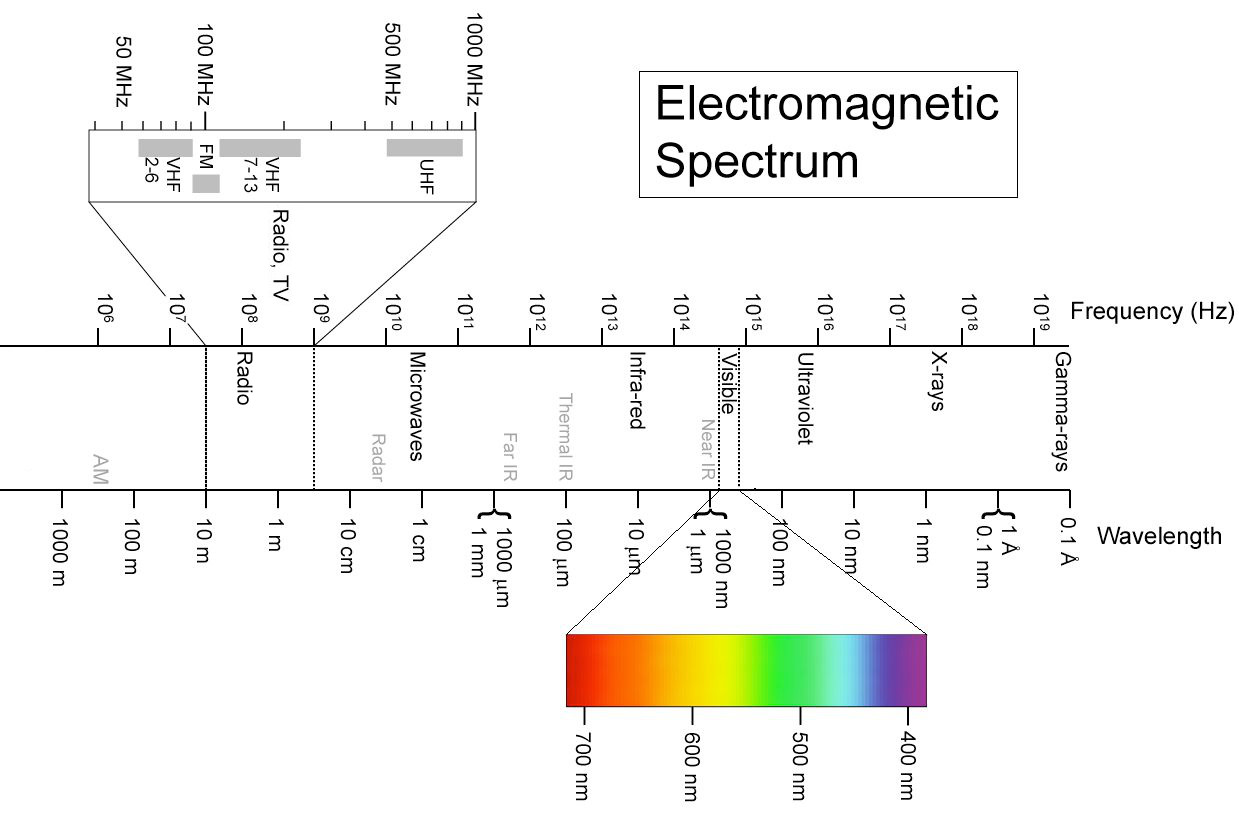
\includegraphics[scale=0.4]{ems.jpg}}
 
\end{enumerate}
 
\section{Lenses}
\paragraph{}
For the rest of the lab, we will use an optics simulator written by Rick Tu, please go to: \url{https://ricktu288.github.io/ray-optics/simulator}. We will use this tool to obtain a better intuition about optics. I have provided you with a couple of ``starter" files located on CourseWorks. Please download these and save them to your desktop, or any other location you can easily access. We will be using these files throughout the lab. Spend a little bit of time getting familiar with the simulator. Scroll over each button at the upper left-hand corner, a pop-up window should appear. Skim through the descriptions provided. Before proceeding, make sure to 1) toggle ``Grid" and ``Snap to Grid" in the ``Settings" menu and 2) toggle ``Rays" under the ``View:" menu.
 
\paragraph{}
Lenses take incoming light and bend it in a way determined by the shape of the lens. There are two basic types of lenses: \textbf{convex} and \textbf{concave}. If parallel rays of light come into the lens, the lens focuses them at one point, called the \textbf{focal point}. This is where the \textbf{image} will form for things which are very far away (like planets, the sun, etc) and from which all the light rays are basically coming in parallel (see the image below).
 
\begin{figure}[ht!]
\begin{center}
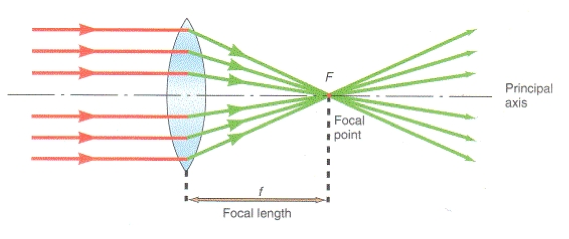
\includegraphics[scale=.6]{Optics_fig1.png}
\label{fig:refracting}
\end{center}
\end{figure}
 
\newpage
\begin{enumerate}
           \item In the optics simulator, locate the ``Open" button, press it to open a file. Navigate to the location where you have saved the files I provided you with. Open the file named ``lab09\_pt1". Axes should appear. The units here are pixels (feel free to ask me about this if you'd like).
           \item We will first insert a lens. Under the ``Tools:" menu, hover over ``Glasses'' and select ``Ideal Lens"
           \item Hover over the following position: x=500, y=100. Click and drag from y=100 to y=0 to create a lens
           \item After creating the lens, a drop down menu appears. The focal length can be found here. What is the focal length? 
           \item Now we will insert light rays. Under the ``Tools:" menu select ``Beam"
           \item Hover over the following position: x=100, y=100. Click and drag from y=100 to y=0 to create a beam of light. Make sure the rays of light are pointed toward the lens.
           \item Describe what you see. What happens to the light rays after passing through the lens? Does this make sense? Take a screenshot of your setup to include in your lab write-up.
           \item Click on the lens for the ``Ideal lens" menu to show up. Change the focal length to -100, you can do this by typing the value into the box.
           \item Now select ``Extended rays" in the ``View:" menu. What are the orange rays? Does it make sense that the light rays converge at that location? Take another screenshot for your lab write-up.
           \item Lenses with a \textit{negative} focal length are known as \textbf{concave} lenses. Lenses with a \textit{positive} focal length are known as \textbf{convex} lenses. What would happen if light rays encountered a lens with a focal length of zero? Is this possible?
           \item The ``Ideal lens" menu has a slider for the focal length. Use this to increase and decrease the focal length. Describe what happens as you move the slider.
\end{enumerate}
 
\section{Testing the Optics}
 
\paragraph{}
For closer objects, light rays from the object to the lens are not necessarily parallel. As a result, the image no longer forms exactly at the focal point of the lens, but rather in a location that depends on the distance from the object to the lens. For the image below, our object (the up arrow on the left marked O) is at P and our image (the down arrow on the right, marked I) is at Q. We label the distances to the object and to the image as: $d_\text{object} = p$ and $d_\text{image} = q$, and the focal length (which we label with the letter $f$) can be calculated from the following equation:
 
\begin{equation}
\frac{1}{f} = \frac{1}{d_\text{object}}+\frac{1}{d_\text{image}} \ .
\end{equation}
 
\begin{figure}[ht!]
\begin{center}
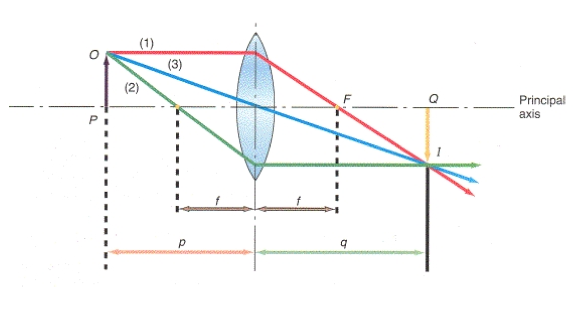
\includegraphics[scale=.6]{Optics_fig2.png}
\end{center}
\end{figure}
 
\paragraph{}
Light is emitted from our object in all directions, and we can follow the path of the light as it goes through the lens (this is called ray tracing). The first ray, (labeled ray (1) in the figure above) shows the light that comes in perpendicular to the lens: as we saw in our first figure, this will go through the focal point on the other side, because it is just like all of the rays that came in parallel from a very distant object. Similarly, if we have light that goes through the focal point, like ray (2), the lens will cause it to come straight out on the other side. From these two lines alone, you can figure out where the image will form based on where these rays cross. We can also trace a third ray, which goes directly through the middle of the lens and does not change its path. This ray should converge with the other two rays at a single point.
 
\paragraph{}
We will now work with a different setup to exercise this new knowledge. Open up ``lab09\_pt2". This is mostly the same setup but now, instead of a beam of light, there is a point source located at x=100, y=60. As you see, light is going in all directions. Using this setup, measure the focal length of this lens and the ones in ``lab09\_pt3" and ``lab09\_pt4". \textbf{NOTE:} Let's pretend we can't just look at what the focal length is... Remember, the focal length of a thin lens is:
 
\begin{equation}
\frac{1}{f} = \frac{1}{d_o}+\frac{1}{d_i} \ ,
\end{equation}
where $d_o$ is the distance from the object to the lens, $d_i$ is the distance from the lens to the image, and $f$ is the focal length. We are still dealing with `pixels' as our units.
 
\begin{enumerate}
           \item Record the data ($d_o$ and $d_i$ for each of your three lenses) and the calculated focal lengths in your notebook. Remember that you should be finding the focal length for each lens by measuring $d_o$ and $d_i$ and then solving for $f$.
           \item Since we can look up the actual focal length of these lenses, what are the \textbf{percent errors} of your ``measured" values? Ask if you aren't sure how to calculate this.
           \item What happens to the focal length if the object is placed at infinity, i.e. if $d_o$ gets very large? What will $d_i$ be in this case? (don't do anything with the optics simulator for this question -- you should be able to solve it just by looking at the equation above).
\end{enumerate}
 
\subsection{Telescopes}
 
\paragraph{}
The two most basic types of telescopes are refracting telescopes, which use lenses, and reflecting telescopes, which use mirrors. Below are diagrams of each type. Both types collect the light from a faraway object in an objective lens or mirror and then bring the light to a focus. A second lens, called the eyepiece, then allows you to view the image formed.
 
\begin{figure}[ht!]
\begin{center}
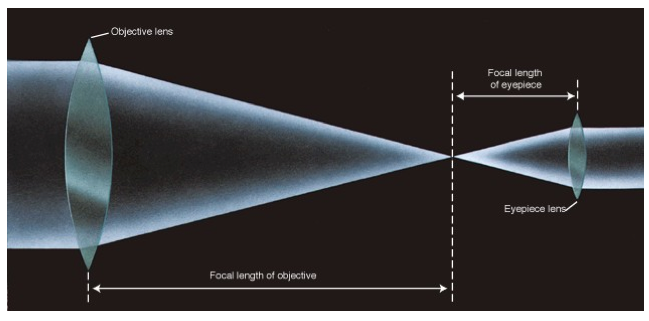
\includegraphics[scale=.4]{Optics_fig3.png}
\caption{A \textit{refracting} telescope.}
\end{center}
\end{figure}
 
\begin{figure}[ht!]
\begin{center}
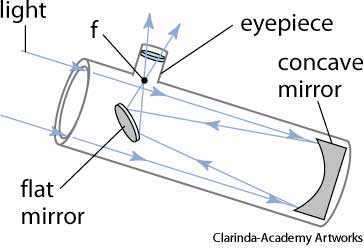
\includegraphics[scale=.6]{Optics_fig4.jpg}
\caption{A \textit{reflecting} telescope.}
\end{center}
\end{figure}
 
\paragraph{}
One of the uses of a telescope is to magnify the object you are viewing, to see it in more detail. Magnification for a refracting telescope is given by the formula:
 
\begin{equation}
M = \frac{f_o}{f_e} \ ,
\end{equation}
where $f_o$ is the focal length of the objective lens (or mirror) and $f_e$ is the focal length of the eyepiece (the second lens).
 
\subsection*{``Building" your own telescope!}
 
\paragraph{}
Now you will use the optics simulator to construct a virtual telescope! You already have everything you need, because an astronomical refracting telescope consists of two convex lenses.
\begin{enumerate}
           \item If you want your telescope to magnify distant objects, should the lens with the longer focal length be the objective or the eyepiece? What will happen if you arrange things the other way around? Recall that the magnification is given by $M = f_o/f_e$.
           \item OK, open up ``telescope\_template" and with the use of 2 \textbf{convex} lenses, try to imitate Figure 1. Play around with the positions of the lenses and their focal lengths. Please let me know if you're unable to replicate Figure 1, I can provide you with an example.
           \item Is the image inverted or upright?
           \item Once you are satisfied with your virtual telescope, take a screenshot for your lab write-up.
           \item What is the magnification of your freshly minted telescope?
\end{enumerate}
 
 
\section{Conclusions}
\begin{enumerate}
\item How many minutes does it take for the Sun's light to reach us on Earth? Please be clear and label your quantities before doing your calculation.
    \begin{enumerate}
    \item From Earh to the the Moon? (in seconds)
    \item From Earth to Mars? (in minutes)
    \item From the Sun to Pluto? (in hours)
    \end{enumerate}
\item Astronomers have to consider many different factors when planning observations of a particular target, including:
           \begin{itemize}
           \item Weather
           \item On-sky position of the target
           \item Brightness of the target
           \item Instrumental limitations
           \end{itemize}
Consider these factors and answer the following.
           \begin{enumerate}
           \item Most major observatories (e.g. the Cerro Tololo Inter-American Observatory in Chile, the Mauna Kea Observatory in Hawaii, and the Kitt Peak National Observatory in Arizona) are located high up on mountains, often in deserts. Why is this?
           \item Will an observatory in Arizona be able to see the same targets as an observatory in Chile? Why or why not?
           \item What do we have to do to take pictures of very faint targets? (Think about nighttime photography in general.) How does Earth's rotation complicate this procedure? Can you think of a way for observatories to account for Earth's rotation?
           \end{enumerate}
 
\item Write down something you learned from this lab. Was anything surprising?
\item Ask a question. 
\end{enumerate}
 
\end{document}